% ============================================================================
% FLARE — MDPI Drones Submission
% ============================================================================
\documentclass[drones,article,submit,moreauthors]{Definitions/mdpi}

\usepackage{siunitx}

% ============================================================================
%                              FRONT MATTER
% ============================================================================

% ORCID identifiers (replace with actual IDs before submission)
\def\orcidauthorA{0009-0001-9498-1016} % K. Zervakis
\def\orcidauthorB{0000-0000-0000-0000} % E. Panagiotopoulos — TODO: replace

\Title{Ranking Inversion in Risk-Parameterised UAV Path Planning for Wildfire Emergency Response}

\TitleCitation{Ranking Inversion in Risk-Parameterised UAV Path Planning for Wildfire Emergency Response}

\Author{Konstantinos Zervakis $^{1,*}$\orcidA{} and Elias Panagiotopoulos $^{1}$\orcidB{}}

\AuthorNames{Konstantinos Zervakis and Elias Panagiotopoulos}

\AuthorCitation{Zervakis, K.; Panagiotopoulos, E.}

\address{%
  $^{1}$ \quad Hellenic Army Academy, Vari, Greece
}

\corres{Correspondence: zervakisai@gmail.com}

% Journal metadata (required by mdpi.cls)
\pubvolume{10}
\issuenum{1}
\articlenumber{0}
\pubyear{2026}
\copyrightyear{2026}
\firstpage{1}
\datereceived{}
\daterevised{}
\dateaccepted{}
\datepublished{}
\hreflink{https://doi.org/10.3390/drones10010000}

% ============================================================================
%                           HIGHLIGHTS (Mandatory for Drones)
% ============================================================================
% MDPI cls checks \@addhighlights for non-empty, then calls \addhighlights
% as a no-argument command (line 1080 of mdpi.cls). Set the internal flag
% directly and redefine the rendering command.
\makeatletter
\gdef\@addhighlights{yes}
\makeatother
\renewcommand{\addhighlights}{%
\begin{itemize}[nosep,leftmargin=*]
  \item Planner orderings by navigation success rate diverge from orderings
        by mission effectiveness---a ranking inversion confirmed across
        450~episodes (Friedman $p < 0.001$).
  \item A single risk coefficient $\rho$ governs the survival--timeliness
        trade-off: higher~$\rho$ increases survival probability at the
        cost of time-induced mission degradation.
  \item Navigation success rate is an insufficient evaluation criterion
        for time-critical disaster-response missions in which delivery
        time determines objective value.
  \item The risk coefficient serves as a principled mission-selection
        parameter, enabling deployment-specific planner configuration.
\end{itemize}
}

% ============================================================================
%                              ABSTRACT
% ============================================================================
\abstract{%
Existing path-planning benchmarks evaluate UAV planners by navigation
success rate---a binary metric that disregards delivery time. This paper
demonstrates that success rate is an insufficient and, in time-critical
disaster-response settings, a misleading evaluation criterion: the
planner with the highest survival probability can yield the lowest
mission effectiveness. This phenomenon is termed \emph{ranking
inversion}. To characterise this effect, we introduce FLARE, a
deterministic benchmark that evaluates five risk-parameterised planners
across 450~episodes on three OpenStreetMap-derived Greek wildfire
scenarios with coupled hazard dynamics (wind-driven fire, structural
collapse, traffic closures). Each planner differs by a single risk
coefficient~$\rho$ that controls sensitivity to a shared hazard cost
map. FLARE quantifies mission impact---medication efficacy, casualty
survival, surveillance freshness---using strictly decreasing functions
of delivery time. Experimental results show that the planner with
the highest success rate (62.7\%) ranks last among adaptive planners
in mission score ($\Delta$Rank~$=$~$-3$), whereas a risk-tolerant
planner achieves the highest mission score despite ranking third in
navigation ($\Delta$Rank~$=$~$+2$; Friedman $p < 0.001$). The
underlying mechanism is identified: higher~$\rho$ induces longer
detours that increase survival probability at the cost of
time-induced mission degradation.
}

\keyword{UAV path planning; wildfire emergency response; ranking inversion; risk-aware planning; mission-impact evaluation; deterministic benchmarking; reproducibility}

% ============================================================================
\begin{document}

% ============================================================================
\section{Introduction}\label{sec:intro}

Natural disasters such as wildfires, earthquakes, and floods generate
rapidly evolving hazard landscapes that severely disrupt ground-based
logistics. In such events, the timely delivery of medical supplies,
situational awareness, and casualty location constitutes the primary
operational objective for emergency
responders~\cite{Erdelj2017,Yucesoy2025}. Traditional relief operations
rely on manned helicopters and ground convoys; however, both modalities
suffer from road network damage, airspace congestion, and limited
scalability~\cite{Rahim2025}. Unmanned aerial vehicles (UAVs) have
emerged as a promising alternative, offering low-cost, rapid-deployment
platforms capable of operating in degraded environments where manned
access is infeasible~\cite{LiWildfire2024,Dradoum2025}.

Over the past decade, extensive research has addressed the UAV path
planning problem across a range of algorithmic families: graph-search
methods such as A*~\cite{Hart1968} and D*~Lite~\cite{Koenig2002},
potential-field approaches~\cite{Khatib1986}, sampling-based planners,
meta-heuristic optimisers, and, more recently, deep reinforcement
learning agents~\cite{Meng2025,Aggarwal2020,Patra2025}. Comprehensive
surveys confirm that path planning remains one of the most actively
studied problems in UAV autonomy, with over 3\,500 publications indexed
between 2000 and 2024~\cite{Bouzid2025,SanchezIbanez2025}. Risk-aware
extensions that modulate edge costs by proximity to hazards have further
improved planner robustness in cluttered
environments~\cite{Zhou2025,Melissaris2025,Karaagac2025}.

Despite these advances, most existing evaluations share a common
limitation: they assess planner performance using navigation-centric
metrics---path length, success rate, or computation time---without
accounting for the temporal value of the mission
objective~\cite{Chen2024fire}. In disaster response, however, mission
effectiveness degrades monotonically with elapsed time: insulin delivered
after 200~steps carries substantially greater clinical value than the
same delivery at 800~steps; a fire-perimeter survey completed before
containment-line decisions is actionable, while one arriving afterwards
is not. Navigation success is therefore a necessary but insufficient
proxy for mission effectiveness.

This distinction is particularly acute in wildfire scenarios, where the
hazard landscape expands continuously. Cellular-automaton (CA) fire
models with wind-directional
spread~\cite{Alexandridis2008,Giannino2025,Sahila2025} generate
time-coupled blocking dynamics that fundamentally alter the
planning problem: corridors that are traversable at step~$t$ may be
impassable at step~$t{+}\Delta t$. Under such conditions, UAV planners
face an intrinsic trade-off between survival probability and delivery
speed. A conservative (high-risk-aversion) planner increases its
likelihood of reaching the goal by circumnavigating hazard zones, but
the resulting temporal penalty may render the completed mission
ineffective. A risk-tolerant planner may attempt shorter routes through
fire fringes, accepting higher collision probability in exchange for
faster arrival. Recent multi-UAV firefighting studies confirm the
complexity of planning under expanding fire
dynamics~\cite{Wang2025fire,Liu2025swarm}, yet none evaluate the
mission-level consequences of the survival--speed trade-off.

This paper identifies and characterises the \emph{ranking inversion}
phenomenon: planner orderings by navigation success rate diverge
systematically from orderings by mission impact score. Across
450~deterministic episodes on three Greek wildfire scenarios, the planner
with the highest survival rate ranks last in mission effectiveness.

The underlying mechanism traces to a single parameter---the risk
coefficient~$\rho \in \mathbb{R}_{\geq 0}$---that governs how strongly
each planner avoids hazards. Higher~$\rho$ amplifies perceived danger,
producing wider detours with higher survival probability.
Lower~$\rho$ discounts risk, permitting shorter-time routes through fire
fringes at the cost of increased collision probability. Risk is not
penalised directly---it is penalised through time-induced mission
degradation:
\begin{equation}
  \rho \;\uparrow\;\; \Rightarrow \;\;
  \text{higher } P(\text{survive}) \;\Rightarrow\;\;
  t \;\uparrow\;\; \Rightarrow \;\;
  M(t) \;\downarrow
\end{equation}
where $t \in \mathbb{N}$ is the delivery step and $M: \mathbb{N} \to [0,1]$
is the strictly decreasing mission score.

\textbf{Contributions.}
\begin{itemize}[nosep,leftmargin=*]
  \item \textbf{FLARE benchmark}: three OSM-derived wildfire scenarios with
    coupled hazard dynamics and time-decaying mission scores, grounded in
    real Greek incidents (2021 Evia, 2023 Evros), enforcing 36~deterministic
    contracts.
  \item \textbf{Risk-parameterised planner suite}: five planners spanning
    static, adaptive, and reactive families, differing solely in~$\rho$.
  \item \textbf{Ranking inversion}: empirical demonstration, supported
    by statistical validation (Friedman $p < 0.001$, Shapley attribution),
    that planner orderings by navigation success rate diverge from orderings
    by mission effectiveness.
\end{itemize}

The remainder is organised as follows: Section~\ref{sec:methods} describes the
benchmark design; Section~\ref{sec:results} presents experiments;
Section~\ref{sec:discussion} interprets findings; Section~\ref{sec:conclusions}
concludes.

\subsection{Related Work}\label{sec:related}

\textbf{UAV path planning in disaster response.}
The deployment of UAVs for disaster relief has expanded rapidly, with
applications spanning medical delivery, search-and-rescue, damage
assessment, and communications
relay~\cite{Erdelj2017,Yucesoy2025,LiWildfire2024}. Path planning
constitutes a central enabling technology for these missions. Classical
graph-search planners---A*~\cite{Hart1968},
D*~Lite~\cite{Koenig2002}---and reactive controllers such as artificial
potential fields (APF)~\cite{Khatib1986} remain widely adopted due to
their determinism and computational tractability. Recent surveys document
a growing trend toward hybrid architectures that combine classical
planning with learning-based
adaptation~\cite{Meng2025,Dradoum2025,Aggarwal2020,Patra2025}. Risk-aware
extensions weight traversal costs by hazard proximity or probabilistic
threat maps~\cite{Zhou2025,Melissaris2025,Karaagac2025,Chen2024fire},
demonstrating improved robustness in uncertain environments. However,
these evaluations employ path-level metrics exclusively: path length,
computation time, or binary success. No existing work evaluates the
\emph{mission-level} consequences of risk sensitivity---an omission
that the present work addresses.

\textbf{Reproducible benchmarking.}
Henderson et al.~\cite{Henderson2018} demonstrated the fragility of
reinforcement-learning evaluations when seeds and hyperparameters are not
controlled. Subsequent best practices now include interquartile mean
(IQM) with bootstrap confidence intervals~\cite{Agarwal2021},
non-parametric Friedman/Wilcoxon rank tests~\cite{Demsar2006}, and
performance profiles~\cite{Dolan2002}. Bonsignorio et
al.~\cite{Bonsignorio2025} advocate published experimental contracts as
a reproducibility mechanism. A recent bibliometric analysis of the UAV
path planning literature confirms that standardised evaluation
protocols remain rare, with fewer than 8\% of studies reporting
seed-controlled deterministic
experiments~\cite{Bouzid2025}. FLARE adopts all four elements:
deterministic replay, IQM, rank tests, and 36~enforceable contracts
verified by 189~automated assertions.

\textbf{Dynamic fire environments.} Cellular-automaton (CA) models with
wind-directional spread~\cite{Alexandridis2008,Giannino2025,Sahila2025}
capture the dominant fire propagation mechanism and have been validated
against satellite-observed burn patterns at landscape
scale~\cite{NatureFire2025}. Multi-UAV
planning under spreading fire has recently attracted attention: Wang et
al.~\cite{Wang2025fire} address multi-target firefighting task
allocation in dynamic forest fire environments, while Liu et
al.~\cite{Liu2025swarm} propose cooperative firefighting strategies
under resource constraints using fire-spread-aware scheduling. Most UAV
path planning benchmarks, however, employ static or randomly toggled
blockages~\cite{Zhao2020}---environments that do not worsen over
time. FLARE's physically motivated dynamics (spreading fire, collapsing
buildings, closing roads) create a \emph{monotonically degrading}
environment, a qualitatively harder and more realistic challenge.

\textbf{The missing evaluation paradigm.} Across all three research
threads---path planning, reproducible benchmarking, and dynamic
environments---existing work shares one critical blind spot:
\emph{time-coupled mission value}. Existing evaluation frameworks count
completions but do not assess their temporal value. By coupling a strictly
decreasing mission score $M(t)$ with expanding hazard dynamics, FLARE
reveals performance trade-offs that success rate alone cannot capture.

% ============================================================================
\section{Materials and Methods}\label{sec:methods}

\subsection{Environment}\label{sec:environment}

FLARE operates on a grid $\mathcal{G} = \{0,\dots,499\}^2$ (${\sim}3$\,m
per cell), extracted from OpenStreetMap tiles~\cite{Boeing2017} of Greek
urban areas. The Gymnasium-compatible~\cite{Towers2025} environment exposes
$|\mathcal{A}|{=}5$ actions (four cardinal moves and stay). A strict timing
contract governs each step: the planner observes the \emph{current}
blocking mask (frozen), selects an action, and only \emph{then} do dynamics
advance (fairness contract FC-2). If fire or debris reaches the agent's
cell after the dynamics update, the episode terminates immediately.

\subsection{Hazard Dynamics}\label{sec:dynamics}

Three coupled layers produce a hazard landscape that worsens monotonically.

\textbf{Wind-driven fire.} Spread follows a cellular automaton on the Moore
neighbourhood~\cite{Alexandridis2008}, modulated by wind direction and land
use. Downwind cells ignite faster; upwind cells are suppressed
(Figure~\ref{fig:wind}). A buffer zone (radius~1) and dense smoke further restrict UAV movement.

\begin{figure}[!htb]
\begin{adjustwidth}{-\extralength}{0cm}
  \centering
  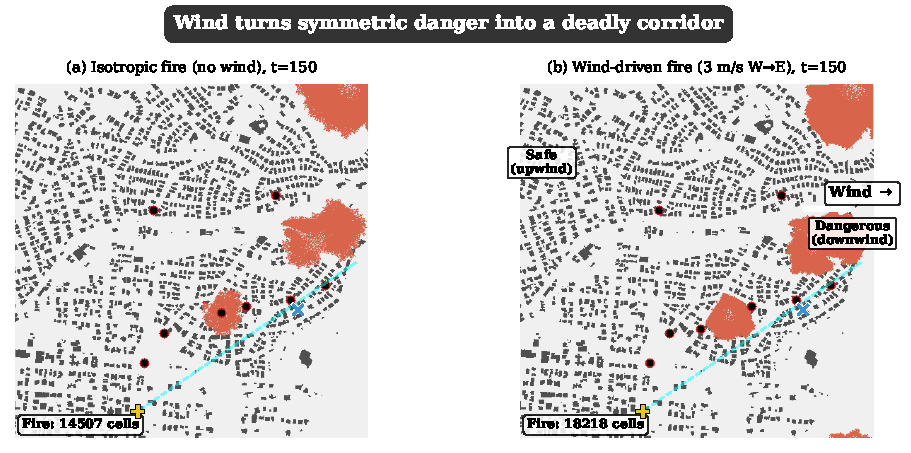
\includegraphics[width=\linewidth]{../figures/wind_driven_fire.pdf}
  \caption{Wind reshapes the hazard geometry. (\textbf{a})~Without wind, fire expands
    symmetrically. (\textbf{b})~At 3\,m/s from the west, fire elongates downwind,
    blocking the direct route while the upwind flank remains passable for
    risk-tolerant planners. Black circles denote dynamic obstacles; blue
    cross denotes the UAV. Penteli, seed~42, $t{=}150$.}
  \label{fig:wind}
\end{adjustwidth}
\end{figure}

\textbf{Structural collapse.} Buildings exposed to fire for
$\tau_c{=}80$~steps collapse with probability $p_d{=}0.6$, scattering
permanent debris. Unlike fire---which burns out---debris
\emph{accumulates}, progressively eliminating detour options
(Figure~\ref{fig:collapse}).

\begin{figure}[!htb]
  \centering
  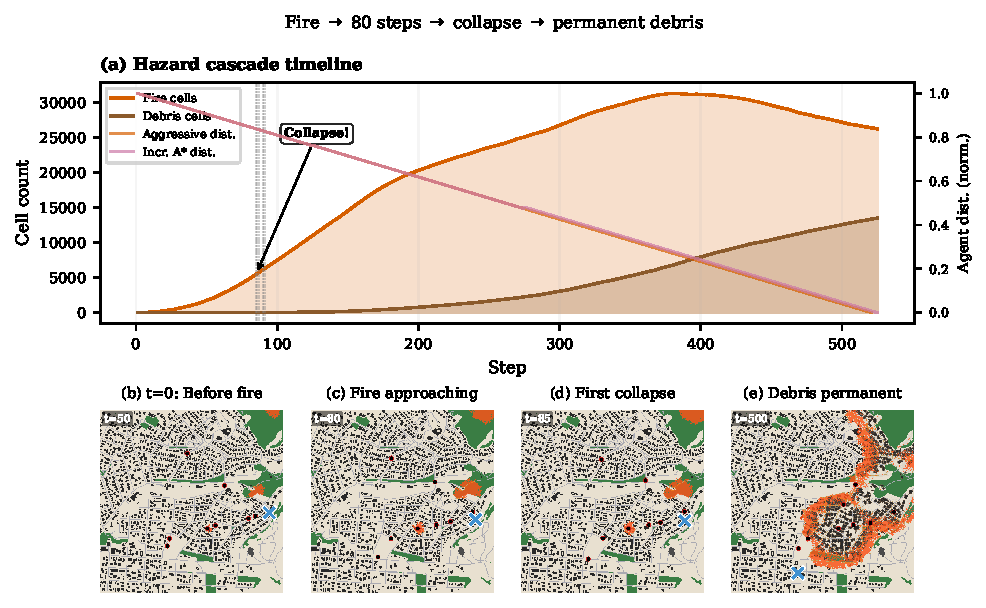
\includegraphics[width=0.95\columnwidth]{../figures/collapse_cascade.pdf}
  \caption{Cascading hazard coupling. (\textbf{a})~Fire peaks then recedes, but
    debris grows permanently. (\textbf{b}--\textbf{e})~Four snapshots trace the cascade
    from clean grid to permanent debris field (Penteli, seed~42).}
  \label{fig:collapse}
\end{figure}

\textbf{Dynamic obstacles.} Moving obstacles patrol the road and maritime
network, blocking UAV movement within a Manhattan buffer (radius~5). The
interaction engine couples fire to traffic: fire proximity closes
segments, creating compound blockages that neither layer produces
alone (Figure~\ref{fig:traffic}).

\begin{figure}[!htb]
\begin{adjustwidth}{-\extralength}{0cm}
  \centering
  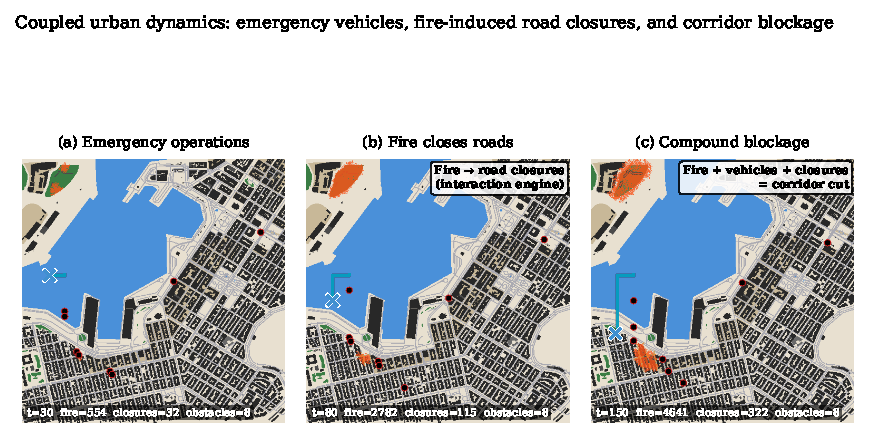
\includegraphics[width=\linewidth]{../figures/traffic_dynamics.pdf}
  \caption{Fire--obstacle coupling (Piraeus, seed~42). (\textbf{a})~Dynamic
    obstacles operate normally at $t{=}30$. (\textbf{b})~Fire triggers segment
    closures by $t{=}80$. (\textbf{c})~At $t{=}150$, fire, closures, and diverted
    obstacles jointly cut the corridor. Black circles denote dynamic
    obstacles; blue cross denotes the UAV.}
  \label{fig:traffic}
\end{adjustwidth}
\end{figure}

\subsection{Risk Cost Map}\label{sec:riskmap}

The perception pipeline maps raw hazards to planner-specific edge costs
in two stages: \emph{risk fusion} and \emph{cost inflation}.

\textbf{Stage 1: Risk fusion.} Five distance-decay layers are fused into a
continuous risk map $R: \mathcal{G} \to [0,1]$ via element-wise max:
\begin{equation}\label{eq:risk}
  R(\mathbf{x}) = \max\bigl(R_f,\; R_s,\; R_t,\; R_b,\; R_{\text{nfz}}\bigr)
\end{equation}
where $R_f{=}[1{-}d_f/r_f]^+$ (fire), $R_s{=}s/2$ (smoke),
$R_t{=}0.6[1{-}d_t/r_t]^+$ (traffic), $R_b{=}0.7[1{-}d_b/r_b]^+$
(debris), and $R_{\text{nfz}} \in \{0, 0.5, 1\}$ (no-fly zones),
for $\mathbf{x} \in \mathcal{G}$, where $d_f, d_t, d_b$ are Euclidean
distance transforms from fire, traffic, and debris with influence radii
$r_f{=}30$, $r_t{=}10$, $r_b{=}8$ cells; $s \in [0,1]$ is smoke
concentration; $[\cdot]^{+}{=}\max(\cdot,0)$. The scaling constants
(0.6, 0.7) are calibrated heuristics reflecting the relative severity
of each hazard layer (insensitive to $\pm 20\%$ perturbation). We use
$\max$ rather than summation so that a single severe hazard dominates
regardless of benign neighbours.

\textbf{Stage 2: Cost inflation.} Each planner inflates its edge cost
using a planner-specific risk coefficient $\rho \in \mathbb{R}_{\geq 0}$:
\begin{equation}\label{eq:cost}
  w(\mathbf{x}) = 1 + \rho \cdot R(\mathbf{x})
\end{equation}

High~$\rho$ amplifies perceived danger, causing wider
detours; low~$\rho$ allows routes through fire fringes.

Figure~\ref{fig:riskperception} illustrates that $\rho$ alone---rather
than the algorithmic family---determines the effective cost landscape:
identical fire state produces five distinct cost surfaces.

\begin{figure}[!htb]
\begin{adjustwidth}{-\extralength}{0cm}
  \centering
  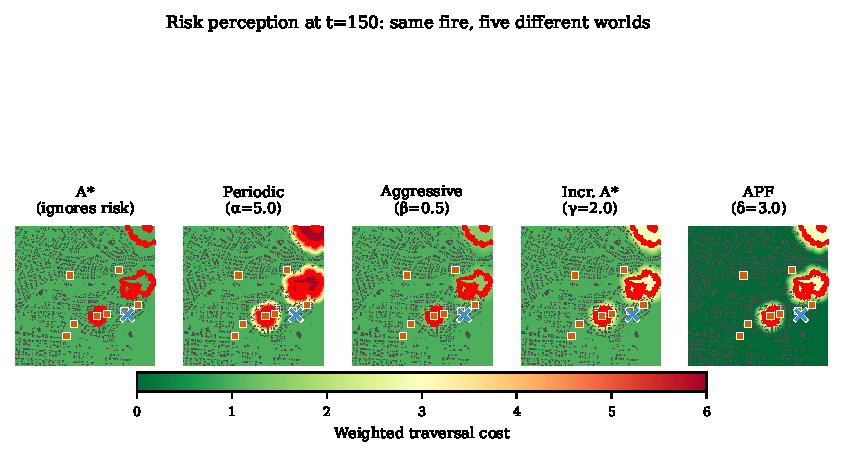
\includegraphics[width=\linewidth]{../figures/risk_perception_5panel.pdf}
  \caption{Planner-specific cost landscapes at $t{=}150$ for identical
    fire state. Each panel shows the inflated edge cost
    $w(\mathbf{x}) = 1 + \rho \cdot R(\mathbf{x})$. A*~($\rho{=}0$)
    perceives uniform cost. Periodic~($\alpha{=}5.0$) inflates fire
    proximity to near-impassable levels. Aggressive~($\beta{=}0.5$)
    applies minimal inflation. The risk coefficient determines the
    effective cost landscape independently of the planning algorithm.}
  \label{fig:riskperception}
\end{adjustwidth}
\end{figure}

\subsection{Planner Suite}\label{sec:planners}

Five planners from three algorithmic families are controlled by a single
coefficient~$\rho$ (Table~\ref{tab:planner_profiles}).

\begin{itemize}[nosep,leftmargin=*]
  \item \textbf{A*}~\cite{Hart1968}: static baseline; plans once, $\rho{=}0$
    (ignores risk).
  \item \textbf{Periodic}: replans every 6~steps, $\alpha{=}5.0$ (risk-averse).
  \item \textbf{Aggressive}: replans on mask change, $\beta{=}0.5$
    (risk-tolerant).
  \item \textbf{Incremental A*} (D*~Lite-inspired~\cite{Koenig2002}): replans on
    path invalidation, $\gamma{=}2.0$.
  \item \textbf{APF}~\cite{Khatib1986}: gradient repulsion, $\delta{=}3.0$.
\end{itemize}

\begin{table}[!htb]
\centering
\caption{Planner profiles and ranking discrepancy. The $\Delta$ column
  quantifies the divergence between navigation and mission rankings:
  the highest-SR planner (Incr.\ A*, Nav.R~\#1) ranks \#4 in mission
  effectiveness, while the highest-MS planner (Aggressive, Ms.R~\#1)
  ranks \#3 in navigation.
  SR = feasible success rate; MS = normalised mission score.}
\label{tab:planner_profiles}
\begin{tabular}{llclrrrrc}
\toprule
\textbf{Planner} & \textbf{Family} & \textbf{Risk Coeff.} & \textbf{Replan Trigger} & \textbf{SR\%} & \textbf{MS} & \textbf{Nav.R} & \textbf{Ms.R} & $\boldsymbol{\Delta}$ \textbf{Rank} \\
\midrule
A* & Static & --- & Never & 0.0 & 0.00 & 5 & 5 & $0$ \\
Periodic & Adaptive & $\alpha{=}5.0$ & Every 6 steps & 55.4 & 0.98 & 2 & 2 & $0$ \\
Aggressive & Adaptive & $\beta{=}0.5$ & On obstacle change & 50.6 & 0.99 & 3 & 1 & $+2$ \\
Incr. A* & Adaptive & $\gamma{=}2.0$ & On path blocked & 62.7 & 0.54 & 1 & 4 & $-3$ \\
APF & Reactive & $\delta{=}3.0$ & Every step (gradient) & 33.7 & 0.57 & 4 & 3 & $+1$ \\
\bottomrule
\end{tabular}
\end{table}

\subsection{Mission Scoring}\label{sec:missions}

Standard benchmarks count successes. FLARE measures the \emph{value} of
each success by defining a mission score $M(t) \in [0,1]$ that is
\emph{strictly decreasing} in delivery time~$t \in \mathbb{N}$
(Figure~\ref{fig:missiondecay}). Three mission types specialise this
framework:

\textbf{Pharma delivery} (Penteli): medication efficacy decays
quadratically, $E(t) = \max(0,\, 1 - (t/T)^2)$, $T{=}T_{\max}$.
The quadratic form reflects pharmaceutical degradation kinetics:
insulin and temperature-sensitive medications retain near-full
potency during an initial plateau before efficacy degrades
sharply as the therapeutic window closes---a profile ill-suited
to linear approximation.

\textbf{Urban rescue} (Piraeus): casualty survival decays exponentially
with fire-coupled amplification:
\begin{equation}\label{eq:survival}
  S_i(t) = \exp\bigl(-\lambda_{\text{eff},i} \cdot t\bigr), \;\;
  \lambda_{\text{eff}} = \lambda_0
  \bigl(1 + \kappa / \max(d_{\text{fire}}, 1)\bigr)
\end{equation}
where $\lambda_0$ is the base decay rate and $\kappa{=}5.0$ is the
fire-coupling constant. Casualties near active fire expire faster, explicitly
rewarding planners willing to enter dangerous zones.
The fire-coupling term $\kappa / d_{\mathrm{fire}}$ captures a
documented triage reality: casualties near an advancing fire
front face compounding threats---heat exposure, smoke inhalation,
structural instability---that accelerate physiological decline
beyond the baseline trauma rate. Consequently, two casualties
of identical severity at the same elapsed time may present
vastly different rescue values depending solely on fire
proximity at the moment of contact.

\textbf{Fire surveillance} (Downtown): data freshness decays linearly,
$F(t) = 1 - t/T$. A fire perimeter map becomes stale as the front advances.
Linear freshness decay is standard in time-critical
intelligence, surveillance, and reconnaissance (ISR)
doctrine, where situational awareness degrades at a
roughly constant rate as the observed scene evolves.

\textbf{Key property.} All three functions share one characteristic: they
are strictly decreasing in~$t$. Every additional step of detour
\emph{destroys mission value}. Cross-scenario comparison uses
per-scenario normalisation (divide by scenario max, then average).

\begin{figure}[!htb]
  \centering
  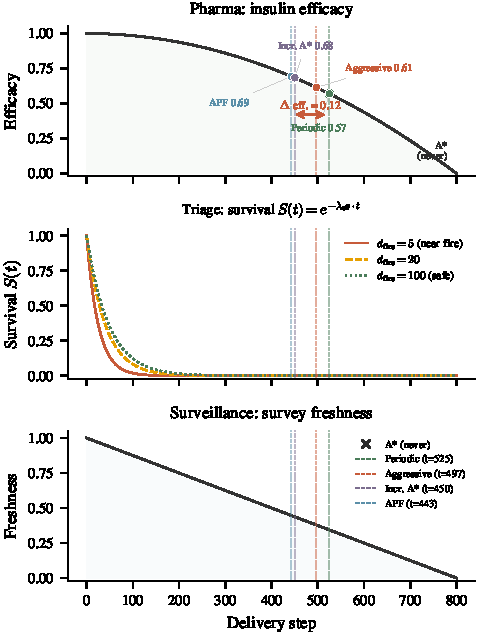
\includegraphics[width=0.95\columnwidth]{../figures/mission_score_decomposition.pdf}
  \caption{Why speed matters. All three mission scores $M(t)$ decay with
    delivery time. The shaded gap between Aggressive (low~$t$) and Periodic
    (high~$t$) quantifies the $M(t)$ cost of a risk-averse detour.}
  \label{fig:missiondecay}
\end{figure}

\subsection{Risk--Time--Mission Coupling}\label{sec:coupling}

The link between risk aversion and mission failure is now explicit.
Increasing~$\rho$ produces safer paths with higher survival probability but
longer travel time~$t$. Because every mission score $M(t)$ is strictly
decreasing in~$t$, the additional travel time directly reduces mission
value. This creates a fundamental trade-off:
\begin{equation}\label{eq:coupling}
  \underbrace{\rho \;\uparrow}_{\text{more risk-averse}}
  \;\;\Longrightarrow\;\;
  \underbrace{t \;\uparrow}_{\text{longer detour}}
  \;\;\Longrightarrow\;\;
  \underbrace{M(t) \;\downarrow}_{\text{worse mission outcome}}
\end{equation}
Crucially, the planner receives only a target coordinate and
a cost map---it has no access to POI locations, decay functions,
or mission-level objectives. The runner orchestrates POI
sequencing externally: upon task completion it issues a new
target, and upon timeout or abandonment it redirects the
planner toward the goal. The ranking inversion is therefore
not an artefact of mission-aware planning logic but an
emergent consequence of the cost-inflation parameter~$\rho$
propagating through path geometry into arrival time and,
ultimately, into mission value.

This coupling is the \emph{mechanism} behind the ranking inversion: the
planner with the highest survival probability is penalised not by
hazards but by the delivery time its detours impose---an inevitable
consequence of any strictly time-decreasing objective.

\subsection{Scenarios}\label{sec:scenarios}

Each scenario is grounded in a real Greek wildfire event
(Table~\ref{tab:scenario_overview}).

\begin{itemize}[nosep,leftmargin=*]
  \item \textbf{Penteli} (Evia 2021): wind-driven fire in a wildland--urban
    interface; the mission is insulin delivery before efficacy degrades.
  \item \textbf{Piraeus} (Rhodes 2023): dense port with structural collapse;
    three casualties with fire-coupled survival.
  \item \textbf{Downtown} (Evros 2023): extreme building density (0.50) with
    NFZ corridors for manned aircraft.
\end{itemize}

Each scenario is paired with a mission type that mirrors the
dominant operational challenge of its historical precedent.
Penteli maps the wildland--urban interface of the 2021 Evia
megafire, where isolated settlements required time-critical
medical resupply by air after road access was severed.
Piraeus reproduces the dense port-adjacent topology of the
2023 Rhodes coastal fires, in which structural collapse and
segment closures compounded fire hazards, stranding casualties
across a fragmented urban grid. Downtown Athens reflects the
2023 Evros megafire---the largest single wildfire in EU
history---where overlapping manned-aircraft corridors imposed
dynamic no-fly zones on unmanned surveillance operations.
These pairings ensure that the decay function, hazard
dynamics, and map topology reinforce one another rather
than varying independently.

\begin{table}[!htb]
\centering
\caption{Scenario overview. Three OSM-based scenarios grounded in real Greek wildfires.}
\label{tab:scenario_overview}
\resizebox{\textwidth}{!}{%
\begin{tabular}{lccc}
\toprule
 & \textbf{Penteli} & \textbf{Piraeus} & \textbf{Downtown} \\
\midrule
Real incident & Evia 2021 & Rhodes 2023 & Evros 2023 \\
Mission & Insulin delivery & Search \& rescue & Fire perimeter survey \\
Service time & 0 (fly-through) & 2 steps (hover) & 3 steps (hover) \\
Score decay & Quadratic & Exponential + fire & Linear \\
Map density & 0.18 & 0.29 & 0.50 \\
Fire ignitions & 2 & 2 & 1 \\
Vehicles & 8 network + 2 patrol & 8 network + 2 patrol & 8 network + 2 patrol \\
NFZ zones & 1 & 1 & 2 \\
Infeasible seeds & 0/30 & 3/30 & 4/30 \\
Key challenge & Wind-driven fire sweeps WUI & Collapse + segment closures & Extreme density + NFZ \\
\bottomrule
\end{tabular}}
\end{table}

\subsection{Reproducibility}\label{sec:reproducibility}

FLARE enforces 36~contracts across 15~families, verified by 189~automated
tests. Key guarantees: bit-identical replay from a single RNG seed (DC-1),
planner-agnostic corridor interdictions (FC-1), frozen hazard state during
planning (FD-3). Infeasible episodes are detected at reset and excluded
uniformly across all planners.

% ============================================================================
\section{Results}\label{sec:results}

\subsection{Experimental Setup}\label{sec:setup}

Five planners $\times$ three scenarios $\times$ 30~seeds yield
450~episodes; 7.8\% are structurally infeasible and excluded. Statistics
follow Agarwal et al.~\cite{Agarwal2021}: IQM with 95\% bootstrap CIs
(10,000~resamples), Wilcoxon signed-rank with Bonferroni correction,
Cliff's delta, and Friedman tests.

\subsection{Navigation Performance}\label{sec:navperf}

A* never succeeds: corridor dynamic obstacles block the reference path before fire
even arrives---a consequence of ignoring risk entirely.
Among adaptive planners, Incremental~A* leads (62.7\% feasible SR),
followed by Periodic (55.4\%), Aggressive (50.6\%), and APF (33.7\%).

Table~\ref{tab:mission_scorecard} disaggregates by scenario with
mission-specific metrics and verdicts. Two patterns stand out:
(i)~Piraeus yields the highest success rates (67--70\%) because its dense
layout provides many alternative routes;
(ii)~Downtown is hardest, with extreme density constraining detours.

\begin{table}[!htb]
\centering
\caption{Per-scenario results with mission-specific metrics.
  $\star$~denotes the highest mission score per scenario;
  \textbf{bold}~denotes the highest success rate. The two markers
  fall on different planners in each scenario, consistent with
  the ranking inversion.}
\label{tab:mission_scorecard}
\begin{tabular}{lrlrl}
\toprule
\textbf{Planner} & \textbf{SR\%} & \textbf{Delivery Step} & \textbf{Mission Metric} & \textbf{Verdict} \\
\midrule
\multicolumn{5}{l}{\textbf{Penteli --- Insulin delivery to fire-isolated village (Evia 2021)}} \\
\midrule
A* & 0 & timeout & 0\% & \textit{Collision with dynamic obstacle} \\
Periodic & 40 & $\sim$514 & 59\% & \textit{Extended detour, efficacy loss} \\
Aggressive & 33 & $\sim$429 & 71\% & \textit{Short route via smoke corridor} \\
Incr. A* & \textbf{53} & $\sim$408 & $\star$ 74\% & \textit{Highest SR, timely delivery} \\
APF & 23 & $\sim$412 & 73\% & \textit{Local-minimum delays} \\
\midrule
\addlinespace[4pt]
\multicolumn{5}{l}{\textbf{Piraeus --- Urban rescue in port district (Rhodes 2023)}} \\
\midrule
A* & 0 & timeout & 0.00 & \textit{Blocked by fire and collapse} \\
Periodic & \textbf{70} & $\sim$477 & 2.78 & \textit{High SR, delayed casualty contact} \\
Aggressive & 67 & $\sim$486 & $\star$ 2.98 & \textit{Early casualty contact} \\
Incr. A* & 67 & $\sim$480 & 1.62 & \textit{Moderate navigation and rescue} \\
APF & 48 & $\sim$392 & 1.82 & \textit{Local-minimum induced delays} \\
\midrule
\addlinespace[4pt]
\multicolumn{5}{l}{\textbf{Downtown --- Fire perimeter survey (Evros 2023)}} \\
\midrule
A* & 0 & timeout & 0\% & \textit{No feasible static path} \\
Periodic & 58 & $\sim$599 & 25\% & \textit{Conservative route, data staleness} \\
Aggressive & 54 & $\sim$563 & 30\% & \textit{Shorter route, moderate risk} \\
Incr. A* & \textbf{69} & $\sim$447 & $\star$ 44\% & \textit{Fastest survey, highest freshness} \\
APF & 31 & $\sim$588 & 26\% & \textit{Gradient drift, slow coverage} \\
\bottomrule
\end{tabular}
\end{table}

\subsection{The Ranking Inversion}\label{sec:ranking}

Table~\ref{tab:planner_profiles} contains the paper's central result.
The $\Delta$~Rank column ($\text{Nav Rank} - \text{Mission Rank}$)
quantifies the discrepancy between navigation and rescue performance.
A \emph{ranking inversion} is defined as the condition
$\arg\max_\pi \text{SR}(\pi) \neq \arg\max_\pi M(\pi)$,
where $\text{SR}$ is feasible success rate and $M$ is normalised mission
score. This condition holds across all three scenarios and is confirmed
by Friedman test ($p < 0.001$), establishing that navigation success
rate does not serve as a reliable proxy for mission effectiveness.

\textbf{High-SR planner, low mission rank.} Incremental~A* ranks~\#1 in
SR but only~\#4 in mission score ($\Delta{=}{-3}$). Its efficient,
minimal replanning reaches the goal with high probability but delivers
medication after significant efficacy loss due to conservative routing.
The low replan count (7.5 mean) indicates that the planner does not
re-evaluate route quality as the fire state evolves.

\textbf{Low-SR planner, high mission rank.} Aggressive Replan ranks~\#3
in SR but~\#1 in mission score ($\Delta{=}{+2}$). Its low coefficient
($\beta{=}0.5$) admits routes through fire fringes: when the planner
survives, medication retains high efficacy ($E(t) > 0.7$) and casualties
remain viable ($S(t) > 0$). Low~$\rho$ yields shorter paths
($t \downarrow$), directly increasing~$M(t)$.

The mechanism follows directly from the coupling in
Section~\ref{sec:coupling}: Aggressive applies $w = 1 + 0.5R$, barely
inflating costs near fire, while Periodic applies $w = 1 + 5.0R$---a
$10\times$ stronger aversion signal that produces substantially longer
detours. The resulting temporal penalty reduces mission value despite
the higher survival probability.
Figure~\ref{fig:scatter}(a) illustrates this effect: planners on the
SR-optimal frontier (right side) fall below the diagonal in mission
score, confirming the ranking discrepancy.

\begin{figure}[!htb]
  \centering
  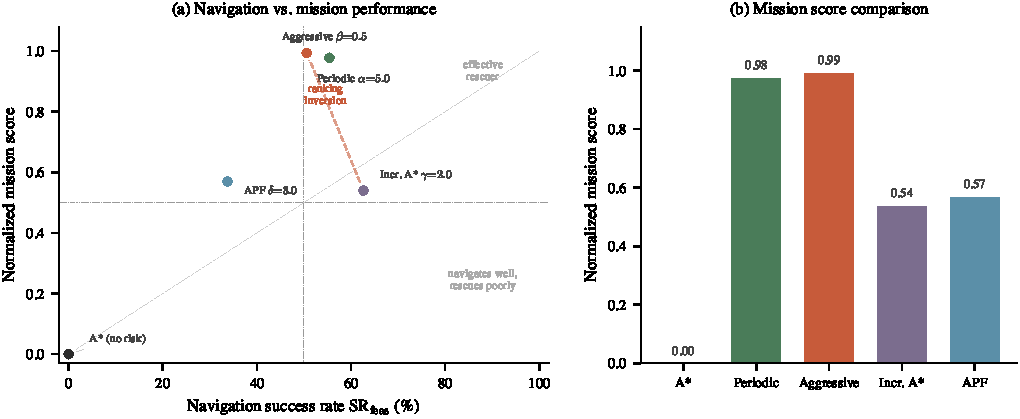
\includegraphics[width=\textwidth]{../figures/mission_impact_scatter_v2.pdf}
  \caption{Ranking inversion between navigation and mission metrics.
    (\textbf{a})~Success rate vs.\ normalised mission score; the dashed
    line connecting Incr.~A* to Aggressive crosses the diagonal,
    indicating divergent orderings. (\textbf{b})~Per-planner mission-score
    decomposition confirms that Aggressive achieves the highest
    aggregate score despite a lower success rate.}
  \label{fig:scatter}
\end{figure}

\subsection{Qualitative Evidence}\label{sec:qualitative}

Figure~\ref{fig:comparison5} provides spatial confirmation of the
ranking inversion. Under identical fire conditions, three planners
produce qualitatively different trajectories. A* terminates upon
collision with a dynamic obstacle at $t{=}78$. Aggressive and Periodic
both complete the mission in comparable step counts (522 vs.\ 524)
but via substantially different paths: Aggressive traverses the smoke
corridor while Periodic circumnavigates the fire perimeter along a
path approximately twice as long. The risk coefficient, rather than
the algorithmic family, determines route geometry.

\begin{figure}[!htb]
  \centering
  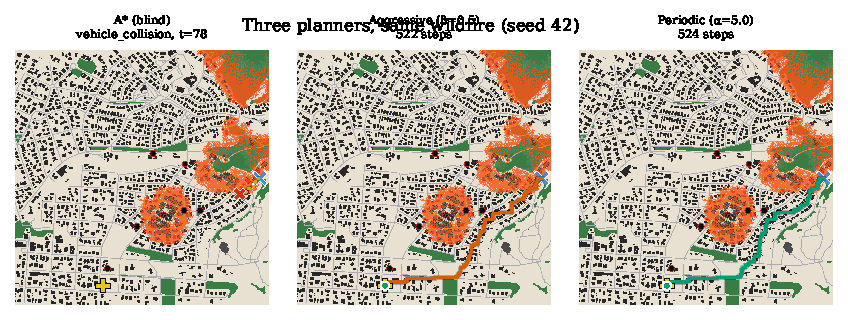
\includegraphics[width=\textwidth]{../figures/trajectory_comparison_5panel.pdf}
  \caption{Trajectory comparison under identical fire conditions
    (Penteli, seed~42). A*~(left) terminates upon collision with a
    dynamic obstacle. Aggressive~(centre) traverses the smoke corridor.
    Periodic~(right) completes a longer detour, arriving with reduced
    medication efficacy. Black circles: dynamic obstacles; blue cross:
    UAV position; yellow cross: target.}
  \label{fig:comparison5}
\end{figure}

\subsection{Statistical Validation}\label{sec:stats}

Wilcoxon tests (Bonferroni-corrected) confirm A* differs from every
adaptive planner ($p < 0.001$). Critically, \emph{no significant
difference} exists between Periodic and Aggressive in SR ($p = 1.0$):
navigation success alone cannot separate them. The discriminator is mission
score: a Friedman test yields $\chi^2(4) = 190.8$, $p < 0.001$,
establishing the ranking inversion as statistically robust
(Table~\ref{tab:stats_summary}).

\begin{table}[!htb]
\centering
\caption{Statistical validation. Friedman confirms ranking differences;
  bootstrap CIs quantify uncertainty.}
\label{tab:stats_summary}
\begin{tabular}{lrrl}
\toprule
\textbf{Test} & \textbf{Statistic} & $\boldsymbol{p}$ & \textbf{Result} \\
\midrule
Friedman (5 planners) & $\chi^2{=}190.8$ & ${<}0.001$ & Planners differ \\
A* vs.\ Adaptive (Wilcoxon) & --- & ${<}0.001$ & All significant \\
A* vs.\ Incr.\ A* (Cliff's $\delta$) & 0.58 & --- & Large effect \\
Incr.\ A* vs.\ APF (Cliff's $\delta$) & 0.27 & --- & Small effect \\
\midrule
\multicolumn{4}{l}{\textit{IQM success rate, 95\% bootstrap CI (10,000 resamples):}} \\
Incr.\ A* & 62.7\% & \multicolumn{2}{l}{[50.9, 74.5]} \\
Periodic & 55.4\% & \multicolumn{2}{l}{[43.1, 67.8]} \\
Aggressive & 50.6\% & \multicolumn{2}{l}{[38.6, 62.6]} \\
APF & 33.7\% & \multicolumn{2}{l}{[22.6, 44.9]} \\
\bottomrule
\end{tabular}
\end{table}

\subsection{Hazard Ablation}\label{sec:ablation}

Isolating dynamics layers reveals their contributions. Fire is the
dominant differentiator: it reduces A* to 0\% while adaptive planners
retain 39--64\%. Traffic alone also eliminates A* but has near-zero
marginal impact on Periodic and Aggressive---their replanning fully
mitigates obstacle blockages. Combined dynamics reduce all planners by
10--20~pp relative to fire alone, confirming non-additive layer interaction.
Road closures grow proportionally with fire (via the
interaction engine); debris accumulates after the collapse delay
($\tau_c{=}80$). Aggressive Replan's timely detours maintain forward
progress; Periodic's risk-averse strategy produces extended stalls---a
direct consequence of the $\rho$--$t$--$M$ coupling.

% ============================================================================
\section{Discussion}\label{sec:discussion}

\subsection{Shapley Attribution}\label{sec:shapley}

Exact Shapley values~\cite{Shapley1953} over coalitions \{fire, traffic,
collapse\} confirm fire as the dominant hazard for all planners. Traffic
degrades A* ($\phi{=}-0.50$) and APF ($\phi{=}-0.25$) but has zero
marginal impact on Periodic and Aggressive---their replanning absorbs
obstacle blockages entirely. Collapse contributes near-zero marginal effect,
subsumed by the fire that triggers it.

In fire-dominated scenarios, the risk coefficient~$\rho$ has greater
influence on mission outcome than replanning frequency; in traffic-heavy
environments, all adaptive planners perform comparably.

\subsection{Risk Coefficient as a Mission-Selection Parameter}\label{sec:knob}

The ranking inversion establishes that no universally optimal planner
exists across mission types. Instead, $\rho$ serves as a principled
mission-selection parameter:

\begin{itemize}[nosep,leftmargin=*]
  \item \textbf{Time-critical delivery} (rescue, medication): $\rho \leq 0.5$.
    Minimise~$t$ to maximise~$M(t)$; accept higher collision probability.
  \item \textbf{Survival-critical operations} (surveillance): $\rho \geq 5.0$.
    Delayed data retains partial value; collision yields $M{=}0$.
\end{itemize}

This finding reframes planner selection: rather than identifying a
single superior algorithm, the appropriate risk coefficient is
determined by the mission-specific relationship between delivery
time and objective value---a relationship that FLARE makes
empirically quantifiable.

\subsection{Limitations}\label{sec:limitations}

Several simplifications constrain the scope of the present study.
FLARE operates on 2D grids without altitude modelling or aerodynamic
constraints. The planner suite comprises classical algorithms; the CA
fire model provides an approximation of real wildfire dynamics. Three
Greek urban scenarios offer focused but not exhaustive geographic
coverage. Risk coefficients are fixed per planner and not adapted
online. The ranking inversion was not predictable \emph{a priori},
as no prior benchmark incorporates time-coupled mission scoring, and
the magnitude ($|\Delta\text{Rank}|{=}3$) required empirical
measurement. Importantly, $\rho$ is not a tunable hyperparameter
but a structural property of each planner's cost function, and
the inversion persists across all three geographically distinct
scenarios. These simplifications are deliberate: the contribution
is the \emph{evaluation paradigm} and the \emph{ranking-inversion
finding}, not the planners themselves.

% ============================================================================
\section{Conclusions}\label{sec:conclusions}

This paper presented FLARE, a deterministic benchmark designed to
evaluate UAV planner performance under time-coupled mission objectives.
Across 450~episodes on three Greek wildfire scenarios, the experimental
results establish a ranking inversion: the planner with the highest
survival probability ranks last in mission score~$M(t)$, because its
detours increase delivery time~$t$ beyond the point at which the
objective retains value. Conversely, a risk-tolerant planner achieves
the highest mission score despite ranking third in navigation success
rate (Friedman $p < 0.001$).

The ranking inversion demonstrates that navigation success rate
constitutes an insufficient evaluation criterion for time-critical
operations, as it can produce orderings that are inversely correlated
with mission effectiveness. The principal implication is methodological:
planner evaluation should incorporate time-dependent mission value
functions rather than relying solely on binary completion metrics.
The risk coefficient~$\rho$ provides a principled parameter for
mission-specific planner selection. The benchmark framework and all
experimental data are publicly available.

Code and data: \url{https://github.com/zervakisai/uavplan}.

% ============================================================================
\vspace{6pt}

\authorcontributions{Conceptualization, K.Z.\ and E.P.; methodology, K.Z.; software, K.Z.; validation, K.Z.\ and E.P.; formal analysis, K.Z.; investigation, K.Z.; resources, K.Z.; data curation, K.Z.; writing---original draft preparation, K.Z.; writing---review and editing, K.Z.\ and E.P.; visualization, K.Z.; supervision, E.P.; project administration, K.Z. All authors have read and agreed to the published version of the manuscript.}

\funding{This research received no external funding.}

\dataavailability{The benchmark code, scenario configurations, and full experimental results are publicly available at \url{https://github.com/zervakisai/uavplan}. Map data are derived from OpenStreetMap~\cite{openstreetmap} under the Open Database License (ODbL).}

\acknowledgments{Map data \copyright~OpenStreetMap contributors (ODbL). Scenarios inspired
by the 2021 Evia wildfire~\cite{effis2021,copernicus_evia2021}, 2023
Rhodes fires~\cite{copernicus_emsr675}, and 2023 Evros
megafire~\cite{copernicus_emsn166,effis2023}. Data from
EFFIS~\cite{effis2021,effis2023} and Copernicus
EMS~\cite{copernicus_evia2021,copernicus_emsr675,copernicus_emsn166}.}

\conflictsofinterest{The authors declare no conflicts of interest.}

\abbreviations{Abbreviations}{The following abbreviations are used in this manuscript:\\

\noindent
\begin{tabular}{@{}ll}
UAV & Unmanned Aerial Vehicle \\
FLARE & Fire-Landscape Adaptive Risk Evaluation \\
SR & Success Rate \\
IQM & Interquartile Mean \\
CI & Confidence Interval \\
CA & Cellular Automaton \\
APF & Artificial Potential Field \\
OSM & OpenStreetMap \\
NFZ & No-Fly Zone \\
RNG & Random Number Generator \\
WUI & Wildland--Urban Interface \\
\end{tabular}
}

\begin{adjustwidth}{-\extralength}{0cm}
\printendnotes[custom]
\reftitle{References}

\bibliographystyle{Definitions/mdpi}
\bibliography{../references}
\end{adjustwidth}

\end{document}
